\section{Koblingsagentens påvirkning på “Good Stuff”}
Som nevnt tidligere vil en automatisk koblingsagent ha stor påvirkning på firmaet som driver “Gi bort dagen”. Først og fremst vil koblingsagenten påvirke i form av redusert ressursbehov på grunn av færre arbeidstimer for å manuelt koble givere med mottakere. I tillegg til lavere ressursbruk, vil en koblingsagent bidra til at “Gi bort dagen” blir et mer fullstendig produkt som er lettere å presentere og markedsføre både til potensielle mottakere og givere, men også til eventuelle økonomiske bidragsytere. 

“Good Stuff” vil, som alle andre bedrifter, avhenge av å være bærekraftig. Dette betyr at de må ha inntekter som tilsvarer eller overstiger kostnadene. I det norske næringslivet er lønnskostnader en av de aller største kostnadsdriverne. Det å kunne minimere disse vil derfor i stor grad bidra til bærekraftighet. En automatisk koblingsagent vil forenkle mye av matchingen mellom mottakere og givere. Det vil ikke være nødvendig med flere ansatte selv om prosjektet vokser da koblingsagenten foreslår gode matcher og mottaker og giver selv kontakter hverandre uten involvering av “Good Stuffs” ansatte. Dette faktum vil være en stor forbedring fra dagens situasjon hvor “Engasjert Byrås” ansatte har brukt mye tid på å manuelt finne gode matcher. Arbeidet var overkommelig det første året, men ettersom konseptet ble mer populært har matchingsarbeidet nærmest blitt uoverkommelig, spesielt tatt i betraktning at “Gi bort dagen” ikke har gitt “Engasjert Byrå” økte inntekter. Det vil naturligvis være nødvendig med ansatte for å drifte og vedlikeholde koblingsagenten. Likevel vil behovet for ansatte være uavhengig av omfanget til prosjektet, noe som bidrar til et mye mer skalerbart produkt. 

Utover muligheten til å påvirke kostnadene til “Good Stuff”, har koblingsagenten også mulighet til å påvirke potensiell inntekt. Gjennom implementering av en automatisk koblingsagent vil “Gi bort dagen”-konseptet bli mye mer komplett. Markedsføringen av konseptet vil forenkles fordi man har noe mer håndfast og strukturert å henvise til. “Gi bort dagen” vil i mye større grad kunne fremstilles som et fullstendig produkt i og med at koblingene er standardiserte og mye mindre påvirket av “Good Stuffs” ansatte. Håpet er at dette vil forenkle prosessen med å selge konseptet til potensielle økonomiske bidragsytere, men også å øke mulighetene for annonsering. Annonsering vil være aktuelt i to former, annonsering og linker til koblingsagenten på eksterne sider som VG.no og adressa.no, men også annonser for andre firmaer på “Gi bort dagens” hjemmeside. Skalerbarhet og standardisering er noen av de viktigste nye egenskapene ved konseptet som følge av en automatisk koblingsagent. Dette er egenskaper som er viktige for eventuelle økonomiske bidragsytere i forbindelse med en beslutning om investering, og dermed bedrer sjansene for flere investorer. 

Utover muligheten for økte sjanser for økonomiske bidragsytere, vil koblingsagenten kunne bidra til nye forretningsmuligheter for “Good Stuff”. For eksempel vil alle mottakere og givere bli bedt om å fylle inn bedriftens/organisasjonens verdier i forbindelse med koblingsprosessen. Dette kan være svært verdifullt for “Good Stuff” da de kan foreslå og tjene penger på rådgiving til firmaer som mangler slike organisasjonsverdier.

En annen inntekstmulighet som koblingsagenten gir er at man som giver må betale en fast avgift for å registrere seg. Denne faste avgiften bør variere avhengig av bedriftens størrelse og omsetning slik at den ikke blir et hinder for å delta, men snarere en symbolsk sum. Et slikt opplegg vil betydelig forbedre “Good Stuffs” bærekraftighet så lenge summen ikke er så høy at den reduserer villigheten til å bidra.

Det er nå pekt på koblingsagentens effekter for Good Stuff. Figur \ref{fig:koblingsagentMuligheter} illustrerer mulighetene som følger av implementering av en koblingsagent og det overordnede resultatet av disse; bærekraftighet.

\begin{center}
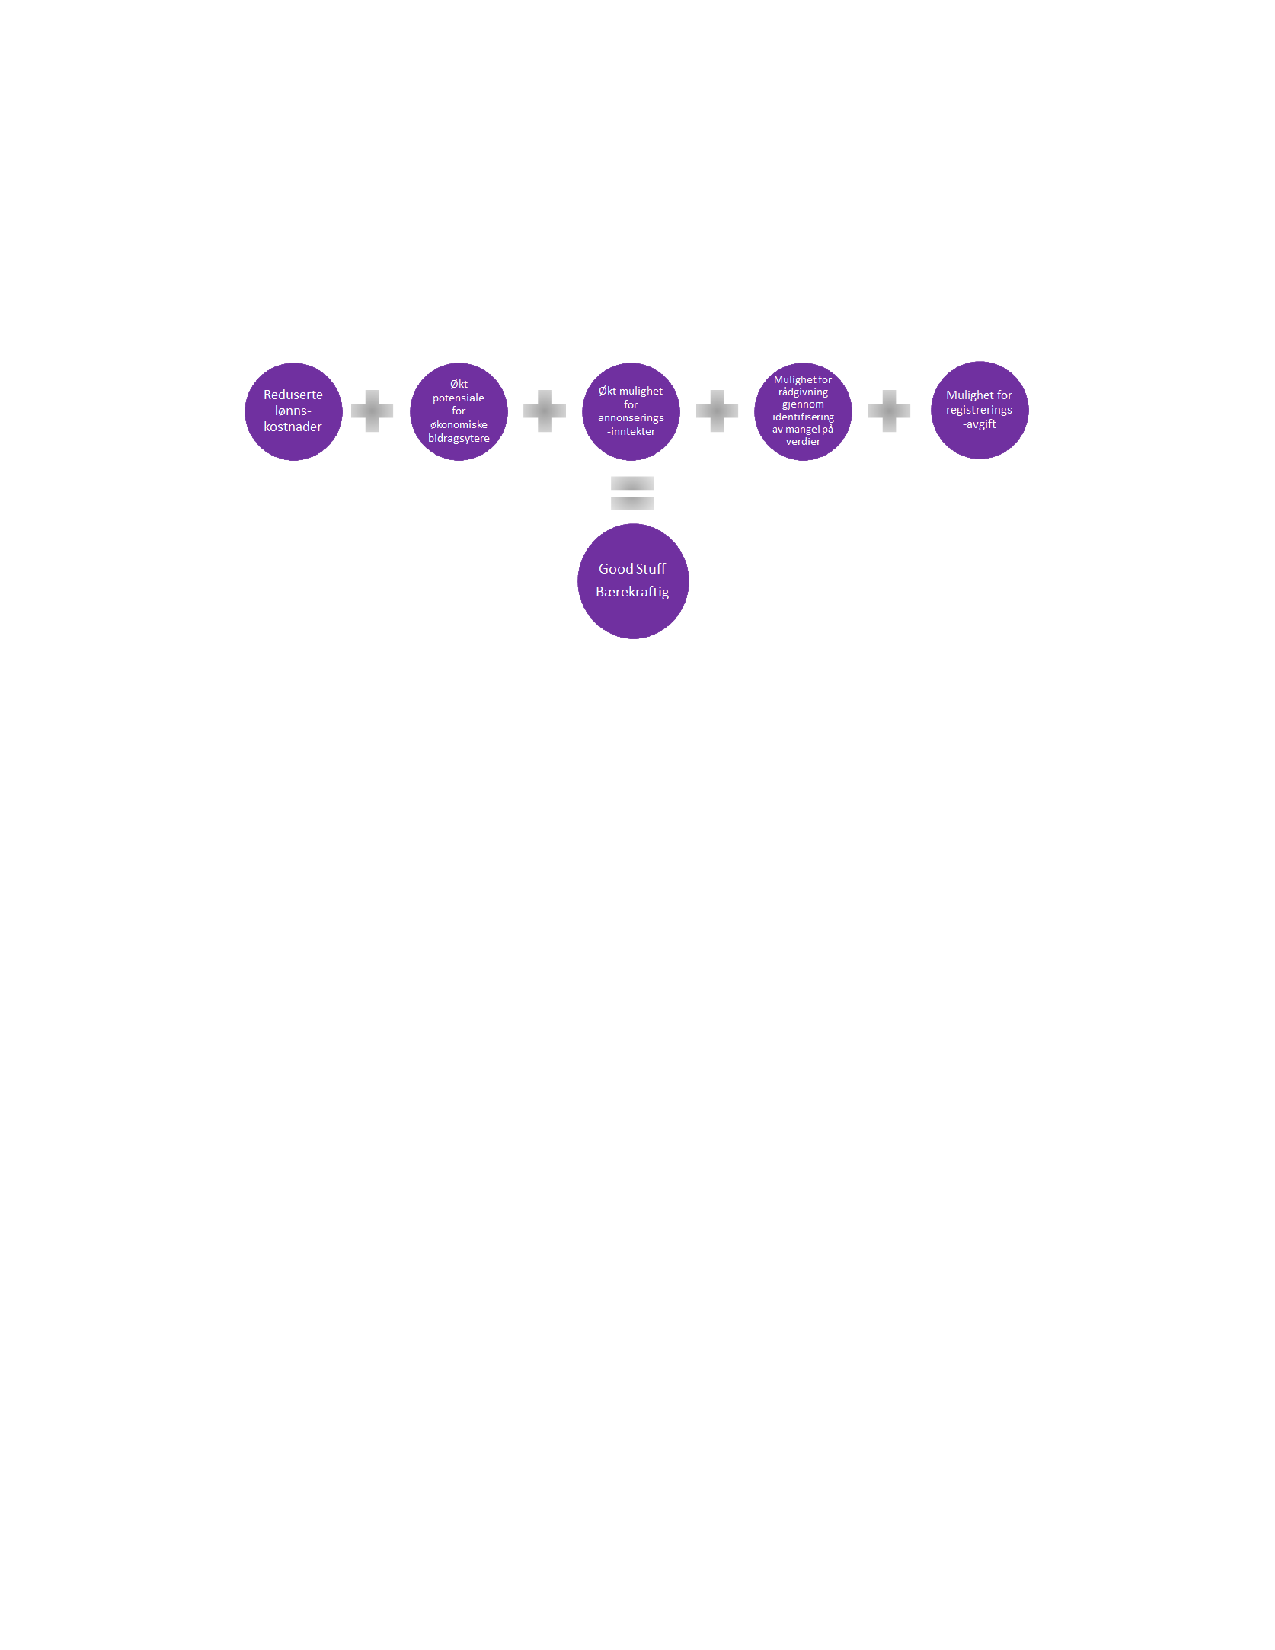
\includegraphics[clip=true, width=1 \textwidth,
trim=0cm 0cm 0cm 0cm]{koblingsagentMuligheter.pdf}
\captionof{figure}{Muligheter og resultat av en automatisk koblingsagent}
\label{fig:koblingsagentMuligheter}
\end{center}

Vi kan dermed konkludere med at en automatisk koblingsagent vil ha en positiv effekt på ``Good Stuff" på flere måter som illustrert i figur \ref{fig:koblingsagentMuligheter}. Uten en automatisering av matchingsarbeidet mellom mottakere og givere i forbindelse med “Gi bort dagen” vil det være vanskelig for “Good Stuff” å videreutvikle prosjektet. På mange måter vil en automatisk koblingsagent derfor være kritisk for “Gi bort dagens”, og dermed også “Good Stuffs” videre suksess.
